\chapter{Design}\vspace{1cm}
Das Kapitel Design beschreibt zunächst die Problemstellung der zugrundeliegenden Arbeit. Zu diesem Zweck wird die bestehende Ausgangssituation aufgezeigt sowie eine kurze Einführung hinsichtlich der Funktionsweise der Anwendung gegeben. Ein Anwendungsfall beschreibt infolge einer dargestellten Benutzerinteraktion die zur Verfügung gestellten Operationen. Im Hauptteil werden die wichtigsten Klassen bezüglich deren Abhängigkeiten und Funktionsweisen vorgestellt. Für die Visualisierung dieser Eigenschaften wurde die graphische Modellierungssprache UML  eingesetzt. Es werden allgemeine Designentscheidungen diskutiert und abschlie\ss end ein Gesamt\"uberblick anhand eines sequentiellen Programmablaufs gegeben.
%
\section{Motivation und Zielsetzung}

Es wurde bereits in den vorherigen Kapiteln erwähnt, dass Energie in der Zukunft eine immer knapper werdende Ressource sein wird. Gerade in der Informatik steigt der Energiekonsum aufgrund neuer Technologien und Online-Services stetig an \cite{Kommey}. Das f\"ur diese Bachelorarbeit entwickelte Programm ist Bestandteil einer Forschung, welche versucht dieses Problem zu l\"osen, indem es mit Hilfe des Paradigmas Accuracy Aware eine energiebewusste Programmierung erm\"oglicht. \\
Die Zielsetzungen waren:
\begin{itemize}
	\item die Fehlerinjektion minimal-invasiv, d.h. mit möglichst wenig Änderungen im Code vornehmen zu müssen.   
	\item Nur einen minimalen Overhead erzeugen, um die Verwendung für große verteilte Systeme (z.B. Hadoop), bei denen neben der Fehlerinjektion zugleich Energiemessungen vorgenommen werden können, zu ermöglichen.
	\item Alle Arten von Datenströmen, wie FileIO oder Network, sollten berücksichtigt werden, weil für ``Accuracy Awareness'' sowohl modifizierte Disk- als auch Network-Hardware simuliert werden soll.
	\item Eine dynamische Regulierung der Fehlerwerte zur Laufzeit. Dem Client sollte es somit m\"oglich sein Fehlerwerte, welche vorher im Programmcode festgelegt wurden, im laufenden Programm modifizieren zu k\"onnen.
\end{itemize}

Das Programm verwendet zun\"achst gew\"ohnliche Streams um Daten einzulesen. Diese werden anschlie\ss end ``verpackt'' und \"uber verschiedene Logiken mit Fehlerwerten injiziert. Danach werden die injizierten Daten für die weitere Verwendung ausgegeben. Die Fehlerinjektion wird über eine Markierung der betroffenen Streams durch Java Annotations\footnote{Metadaten} im Quelltext eingeleitet. Jeder markierte Stream wird somit als fehlerbehaftet gekennzeichnet und bekommt von Beginn an Fehlerwerte zugewiesen. Für die Markierungen wurde eine selbstdefinierte Annotation mit dem Namen \courier{FaultInj} verwendet. Die Fehlerwerte sind durch die vier Parameter ID, Fehlerrate, Fehlertyp und die Gr\"o\ss e eines fehlerbehafteten Datenblocks definiert. Ziel der Fehlerinjektion ist es, die eingelesen Daten mittels diesen konkreten Fehlerwerten und diversen Injektionsstrategien manipulieren zu k\"onnen. F\"ur die Fehlerinjektion war es zusätzlich notwendig, auch mehrere Markierungen/Annotationen mit verschiedenen Werten f\"ur einen Stream definieren zu k\"onnen. 

\section{Benutzerinteraktion}
Die Benutzerinteraktion wurde sehr übersichtlich gestaltet, um den Client eine m\"oglichst kompakte, intuitive Bedienbarkeit zur Verfügung zu stellen. F\"ur den Anwender wurde deshalb eine Schnittstelle mit dem MBean Server kreiert (Siehe dazu Abschnitt \ref{controller}), welche ausschlie\ss lich vier unterschiedliche Funktionalitäten anbietet. \\
In Abbildung \ref{AnFallDia} ist diese Benutzerinteraktion als Anwendungsfalldiagramm bzw. Nutzfalldiagramm dargestellt. Die ersten beiden Operationen der Anwendung mit ähnlicher Funktionalität, geben alle Fehlerwerte respektive die ID's der annotierten Streams zurück. Dies ist insbesondere von Vorteil, wenn später die Fehlerwerte geändert werden sollen und die eindeutige ID des Streams nicht bekannt ist. \\
Um die Fehlerwerte der einzelnen Streams ändern zu können, gibt es eine Methode die in Abbildung \ref{AnFallDia} unter ``Fehlerwerte \"andern'' zu finden ist. Die Änderungsmöglichkeiten umfassen die Fehlerrate, Fehlertyp und die grö\ss e des Datenblocks. Die ID dient zur Zuordnung der Fehlerwerte und kann ausschlie\ss lich im Programmcode ver\"andert werden.\\
Die wichtigste Funktion hat den Namen \courier{runInjection} und ist in Abbildung \ref{AnFallDia} als ``Injektion durchführen'' dargestellt. Für diese Funktion lassen sich zwei Varianten auswählen. Die erste Variante ist für eine Dateiinjektion definiert und benötigt lediglich den Dateipfad. Die zweite Variante verlangt einen Java \courier{InputStream} um allgemeine Datenströme zu verarbeiten. Nach dem Laden der Daten wird durch diese Funktion die eigentliche Fehlerinjektion und die Datenausgabe veranlasst.\\
Für die Datenausgabe sind ebenfalls zwei Wahlmöglichkeiten vorhanden, deren genaue Differenzierung im weiteren Verlauf dieses Kapitels erläutert wird.

\begin{figure}[!htb]
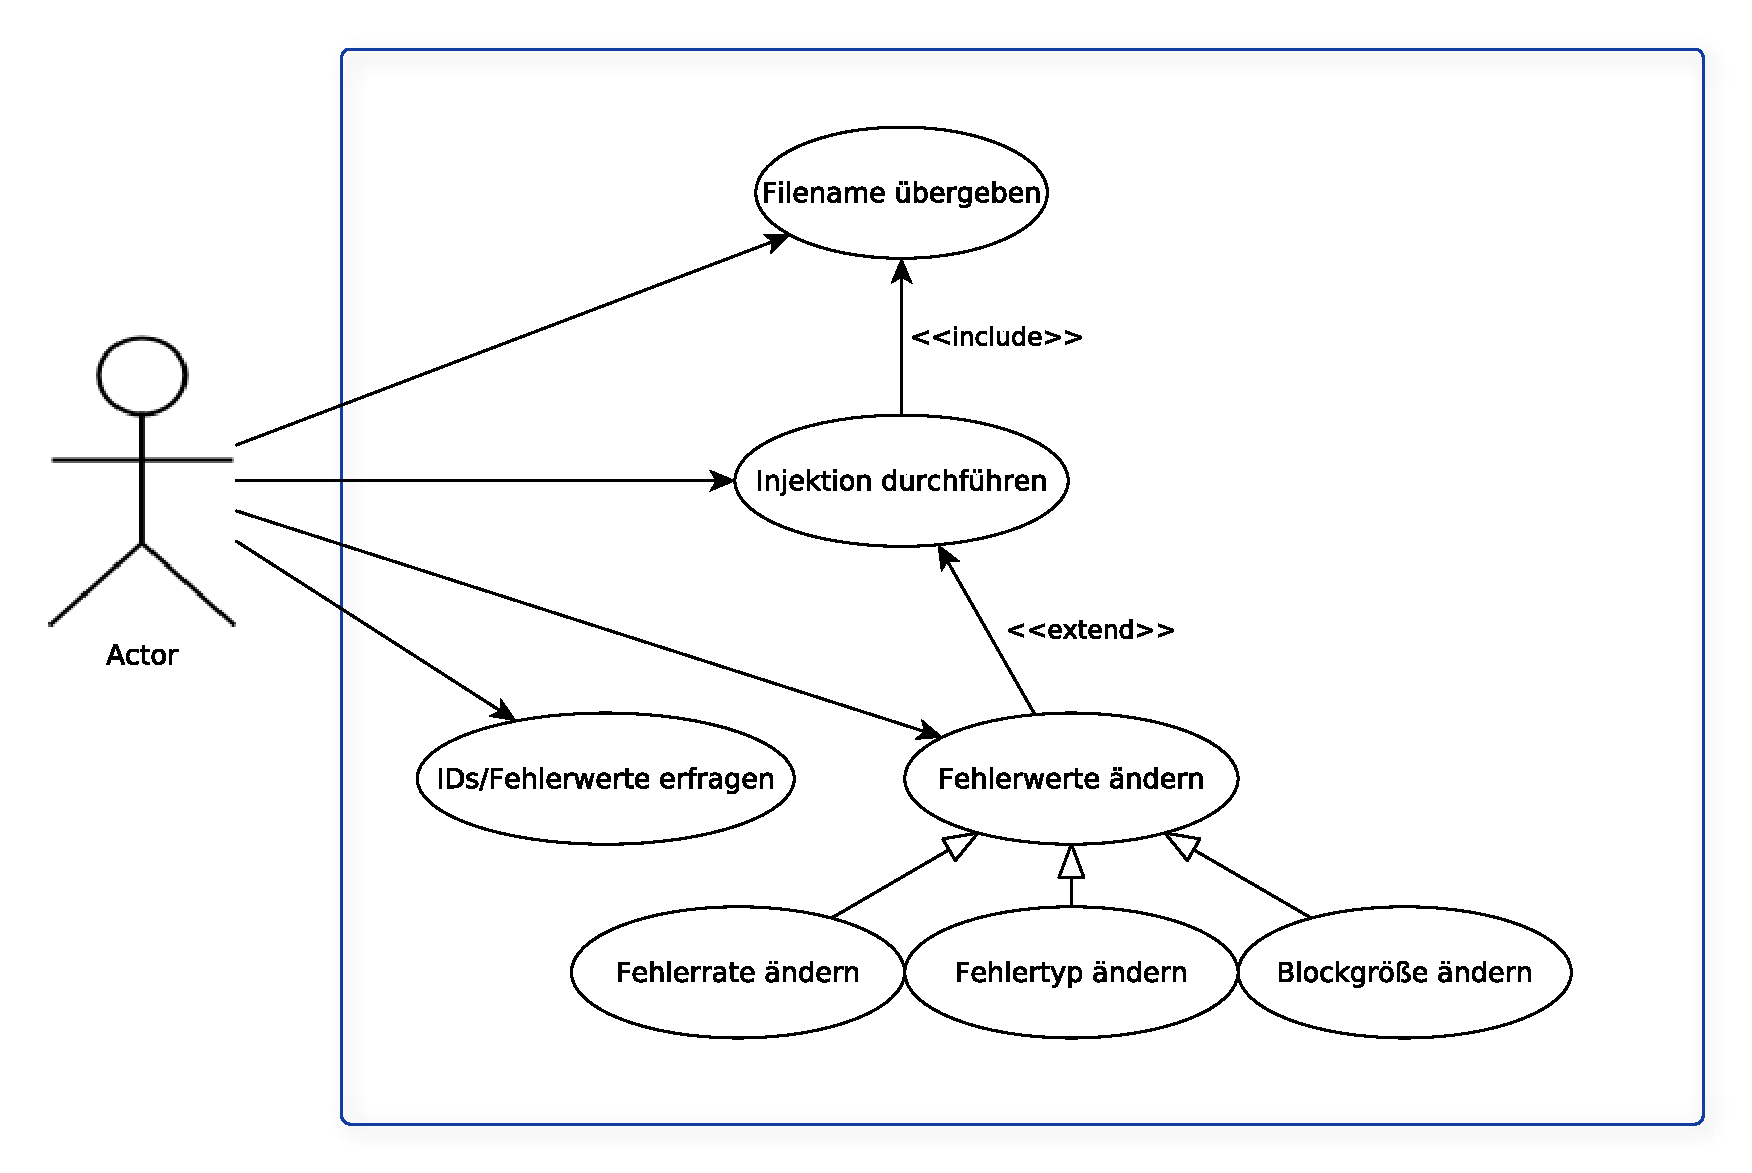
\includegraphics[scale=0.55]{graphics/Anwendungsfalldiagramm.eps}
\centering
 \caption[Anwendungsfalldiagramm]{Anwendungsfalldiagramm}
 \label{AnFallDia}
\end{figure}


\section{Klassendesign \& -abhängigkeiten}
%
Die Klassenhierarchie der zugrunde liegenden Anwendung st\"utzt sich auf den folgenden vier S\"aulen, welche das Grundgerüst bzw. die Hauptfunktionalität der Applikation bilden. Ein wesentliches Ziel war es, die Anforderungen der Modularit\"at zu erf\"ullen. Die Anwendung sollte für eventuelle Erweiterungen m\"oglichst flexibel und gut strukturiert bleiben.
%
	\begin{itemize}
		\item StreamProcesser : Einlesen und Ausgabe der Daten, Start der Fehlerinjektion
		\item InjectionStrategy : Oberklasse der Injektionsstrategien
		\item AddRunTimeAnnotation : Dynamische Modifikation der Annotationen
		\item Controller : Steurerung aller Funktionen
	\end{itemize}	 
%
\subsection{StreamProcessor}

Der \courier{StreamProcessor} ist das Herzst\"uck der Anwendung. Alle Daten die es zu manipulieren gilt, werden an diese Klasse übergeben. Die für das Einlesen der Daten notwenigen Streams sind in der Klassendefinition als globale Variablen vorgesehen. Dies bedeutet auch, dass die Fehlermarkierungen durch die \courier{FaultInj} bzw. mehrere Markierungen durch eine \courier{FaultInjects} Annotation, ausschlie\ss lich global vorgenommen werden können.\\ 
Der \courier{StreamProcessor} zerlegt einen Datenstream in einzelne Bytes, um sie anschlie\ss end der Klasse \courier{Context} zu übergeben. Die Klasse \courier{Context} verwaltet die Daten zusammen mit deren Fehlerwerte, falls jene definiert wurden. Die Implementierung erlaubt es an dieser Stelle auch mehrere Datens\"atze verschiedener Streams durch ein \courier{Context} Objekt verwalten zu lassen. Für jeden Datensatz wird eine eindeutige ID zur Unterscheidung festgelegt. Einzige Prämisse für die Nutzung dieser Datenverwaltung ist die Serialisierbarkeit der Daten, um einen Netzwerktransfer zu erm\"oglichen.\\
Nach dem Einlesevorgang wird über den \courier{StreamProcessor} die Fehlerinjektion veranlasst. Bereits während des Einlesens wurden für jeden Datensatz, anhand der ID des markierten Streams, die Fehlerwerte registriert. Der \courier{StreamProcessor }startet nun die Fehlerinjektion über seine Instanz der Klasse \courier{Context}. Diese bestimmt anhand des Fehlertyps die notwendige Injektions-Strategie. Ist für einen Datensatz kein Strategie vorhanden bleibt dieser unberührt und eine Fehlermeldung wird ausgegeben. Für die konkrete Fehlerinjektion wurde ein Strategy Pattern in leicht abgewandelter Form verwendet. \\
Die aktuelle Implementierung sieht nach der Fehlerinjektion die Datenausgabe in eine Datei vor. Zu diesem Zweck wurde eine innere Klasse \courier{Reducer} implementiert. Sie ist f\"ur die Erstellung der neuen Dateien zust\"andig und bietet hierfür zwei verschiedene Ausgabevarianten an. Per Default wird ein \courier{FileChannel} für die Ausgabe verwendet. Durch eine zusätzliche Funktion kann der Ausgabestream vom Client, zu einem \courier{ObjectOutputStream} geändert werden. Dadurch wird eine persistente Objektspeicherung ermöglicht. Nach diesem Schritt wird durch alle Datens\"atze iteriert und die Daten in die neuen Dateien geschrieben. Diese Struktur ist in Abbildung \ref{FileProcessorUML} als UML-Klassendiagramm dargestellt.

\begin{figure}[!htb] 
\centering
		\umlDiagram[box=,border,sizeX=12cm,sizeY=10cm,ref=pack]{		
			\umlClass[pos=\umlTop{pack}, stereotype=Class, posDelta={0, -10},
				refpoint=t]{StreamProcessor}{}{}
			\umlClass[pos=\umlTop{pack}, stereotype=Class, posDelta={0, -1},
				refpoint=t]{Context}{}{}
			\umlClass[pos=\umlTopRight{pack}, stereotype=Abstract Class, posDelta={-6,-1},
				refpoint=t]{InjectionStrategy}{}{}	
			\umlClass[pos=\umlLeft{pack}, stereotype=Class, posDelta={4, 2},
				refpoint=t]{Reducer}{}{}	
			\umlClass[pos=\umlRight{pack}, stereotype=Annotation, posDelta={-5, 2},
				refpoint=t]{FaultInj}{}{}
			\umlClass[pos=\umlBottom{pack}, stereotype=Annotation, posDelta={0, 6},
				refpoint=t]{FaultInjects}{}{}																	\umlInner{Reducer}{StreamProcessor}
			\umlInstance{StreamProcessor}{FaultInj}	
			\umlInstance{StreamProcessor}{FaultInjects}
			\umlInstance{StreamProcessor}{Context}
			\umlInstance{Context}{InjectionStrategy}									
		}% End of diagram
%		\captionsetup{list=false}
	\caption{UML StreamProcessor}
 	\label{FileProcessorUML}
\end{figure}

\subsection*{Exkurs: Klasse Context}

Bisher wurde häufig die Klasse \courier{Context} erwähnt, welche die eingelesenen Daten verwaltet und  Fehler in die enthaltenen Datensätze einbaut. Um diese Aufgabe zu erfüllen, muss die Klasse \courier{Context} zunächst für jeden Datensatz die erforderliche Injektionslogik bestimmen. Die Injektionslogiken wurden durch eine Form des Strategy Patterns \cite{GammaEtAl00} in die Implementierung integriert.\\
Die Klasse \courier{Context} trifft die Auswahl der konkreten Injektionsstrategie anhand des Fehlertyps des jeweiligen Datensatzes. Eine abstrakte Klasse repräsentiert die allgemeinste Strategie. Sie kann flexibel von den beschriebenen Logiken in den folgenden Abschnitten erweitert/überschrieben werden. Die verschiedenen Strategien sind als einzelne Module definiert, die problemlos durch neue Klassen erg\"anzt werden können. Wenn die richtige Strategie gefunden wurde, kann die Injektion mit den entsprechenden Fehlerwerten gestartet werden.
%
\subsection{Fehlerwerte}
Fehlerwerte sind im Programmcode als Annotationen darstellt. Ein Stream kann dabei auch mit mehreren Annotationen versehen werden. Der Fehlerwert besteht immer aus den folgenden vier Komponenten:

\begin{itemize}
	\item ID: Die ID ist ein eindeutiger Wert zur Unterscheidung bzw. Identifikation der einzelnen Streams. Soll ein Fehlerwert dynamisch ver\"andert werden, wird dieser \"uber die ID angesprochen. Sie wird dementsprechend in der Implementierung gesetzt und kann w\"ahrend der Laufzeit nicht ver\"andert werden.
	\item Type: Der Fehlertyp wird \"uber den Parameter \courier{type} angesprochen. Er repr\"asentiert die Fehlerlogik die angewendet werden soll. Als m\"ogliche Typen stehen in dieser Version der Anwendung RANDOM, LOSS, ZERO, BITFLIP, BITFLIPB, NONE zu Verf\"ugung. Auf deren genauere Bedeutung wird in den folgenden Abschnitten der konkreten Logiken eingegangen.
	\item Rate: Die Fehlerrate ist eine Gleitkommazahl doppelter Genauigkeit und liegt zwischen 0 und 1. Sie gibt die Wahrscheinlichkeit der Injektion eines Blocks oder Bits an. Die Werte stehen für 0\% bis 100\% und flie\ss en in die Berechnung einer Zufallsfunktion ein. Diese  erstellt auf Grundlage der statischen Methode \courier{random} aus der Klasse \courier{Math} einen Zufallswert und setzt diesen in Relation zu der Fehlerrate. Das Ergbnis der Berechnung liefert die Entscheidung über die Injektion eines Blocks oder Bits, abhängig von der konkreten Strategie. Bei einer Fehlerrate von 1 würden demnach alle Blöcke oder Bits injiziert werden.
	\item Blocksize: Die Blockgr\"o\ss e bestimmt die Anzahl der zu injizierenden Bytes, die in einen Block gepackt werden sollen. Bis auf die einfache Bitflip Strategie sind alle Injektionsstrategien auf den Blocksize Parameter angewiesen. Die eben beschriebene Zufallsfunktion arbeitet f\"ur diese Logiken auf der Blockebene. Das hei\ss t die Zufallsentscheidung der Injektion wird nicht f\"ur einzelne Bytes, sondern f\"ur den gesamten Block getroffen.
\end{itemize}

\label{strats}
\subsection{Injektions-Strategie}

Die abstrakte Klasse \courier{InjectionStrategy} wurde als Oberklasse für alle konkreten Strategien definiert. Sie enthält keine eigene Injektionslogik, fordert aber die Implementierung einer Injektionslogik von ihren Unterklassen. Sie stellt ebenso die Zufallsfunktion als auch die Fehlerwerte für ihre Unterklassen zur Verfügung. In Abbildung \ref{StrategyUML} wurde dieses Muster, zuzügliche der Verbindung zur Klasse \courier{Context}, modelliert.

\begin{figure}[!htb] 
\centering
		\umlDiagram[box=,border,sizeX=12cm,sizeY=14cm,ref=pack]{	
			\umlClass[pos=\umlTop{pack}, stereotype=Class, posDelta={0, -1},
				refpoint=t]{Context}{}{}	
			\umlClass[pos=\umlTop{pack}, stereotype=Abstract Class, posDelta={0, -8},
				refpoint=t]{InjectionStrategy}{
					\umlAttribute[visibility=\# , type=FaultValue{[]}]{faults}				
				}{
					\umlMethod[visibility=+, type=void]{\textit{runInjection}}{}
					\umlMethod[visibility=\# , type=boolean]{isInject}{double}				
				}
			\umlClass[pos=\umlLeft{pack}, stereotype=Class, posDelta={5.5, 0},
				refpoint=t]{StrategyBitflip}{}{
					\umlMethod[visibility=+, type=void]{runInjection}{}				
				}
			\umlClass[pos=\umlRight{pack}, stereotype=Class, posDelta={-5.5, 0},
				refpoint=t]{StrategyBitflipB}{}{
					\umlMethod[visibility=+, type=void]{runInjection}{}					
				}	
			\umlClass[pos=\umlBottomLeft{pack}, stereotype=Class, posDelta={7, 7},
				refpoint=t]{StrategyLoss}{}{
					\umlMethod[visibility=+, type=void]{runInjection}{}					
				}	
			\umlClass[pos=\umlBottomRight{pack}, stereotype=Class, posDelta={-7, 7},
				refpoint=t]{StrategyRandom}{}{
					\umlMethod[visibility=+, type=void]{runInjection}{}					
				}
			\umlClass[pos=\umlBottom{pack}, stereotype=Class, posDelta={0, 7},
				refpoint=t]{...}{}{
					\umlMethod[visibility=+, type=void]{runInjection}{}					
				}				
			\umlInstance{Context}{InjectionStrategy}									
			\umlSubclass{InjectionStrategy}{StrategyBitflip}	
			\umlSubclass{InjectionStrategy}{StrategyBitflipB}
			\umlSubclass{InjectionStrategy}{...}	
			\umlSubclass{InjectionStrategy}{StrategyLoss}
			\umlSubclass{InjectionStrategy}{StrategyRandom}											
		}% End of diagram
	%	\captionsetup{list=false}
	\caption[UML Strategy Pattern]{UML Strategy Pattern}
 	\label{StrategyUML}
\end{figure}



\subsubsection{Strategie Bitflip}

Die erste Strategie tr\"agt den Namen Bitflip und ist in der Regel das aufwendigste Verfahren. Grund daf\"ur ist die individuelle Verwendung der Zufallsfunktion f\"ur jedes einzelne Bit. Auch die Datenmanipulation muss, auf Grundlage des Resultats dieser Funktion entsprechend h\"aufig ausgef\"uhrt werden. Wie der Name Bitflip schon verrät, werden bei dieser Strategie Bits lediglich umgedreht\footnote{flip: 0 zu 1 und 1 zu 0}. Im folgenden Beispiel wurden durch die Zufallsfunktion, die Bits an den Positionen 3,4 und 7 ausgew\"ahlt und entsprechend injiziert. \\

\psline[linecolor=red,linewidth=.1cm,
doublesep=1.5pt]{->}(5.2,1.5)(5.2,0)
\psline[linecolor=red,linewidth=.1cm,
doublesep=1.5pt]{->}(6.8,1.5)(6.8,0)
\psline[linecolor=red,linewidth=.1cm,
doublesep=1.5pt]{->}(11.5,1.5)(11.5,0)
\psline[linecolor=red,linewidth=.1cm,
doublesep=1.5pt]{->}(25.5,1.5)(25.5,0)
\psline[linecolor=red,linewidth=.1cm,
doublesep=1.5pt]{->}(27.1,1.5)(27.1,0)
\psline[linecolor=red,linewidth=.1cm,
doublesep=1.5pt]{->}(31.8,1.5)(31.8,0)


$\dots$
\begin{tabular}{|c|c|c|c|c|c|c|c|}
\hline
0 & 1 & 0 & 0 & 0 & 1 & 1 & 1 \\\hline
\end{tabular}
$\dots$
\psline[linewidth=.1cm]{->}(0.5,0)(4,0)
\hspace{2cm}$\dots$
\begin{tabular}{|c|c|c|c|c|c|c|c|}
\hline
0 & 1 & 1 & 1 & 0 & 1 & 0 & 1 \\\hline
\end{tabular}
$\dots$

\subsubsection{Strategie BitflipB}

Diese Strategie funktioniert analog zum normalen Bitflip. Einzige Ausnahmen sind die Bearbeitung ganzer Bytes statt einzelner Bits sowie die Möglichkeit der Blockverarbeitung. Die Zufallsfunktion entscheidet diesmal individuell f\"ur jeden Block \"uber dessen Injektion. Wird ein Block zur Injektion ausgew\"ahlt, werden s\"amtliche Bits der darin enthaltenen Bytes gedreht. Wird der Block nicht ausgew\"ahlt, bleiben die Bytes komplett erhalten.\\

$\dots$
\begin{tabular}{|c|c|c|c|c|c|c|c|}
\hline
0 & 1 & 0 & 0 & 0 & 1 & 1 & 1 \\\hline
\end{tabular}
$\dots$
\psline[linewidth=.1cm]{->}(0.5,0)(4,0)
\hspace{2cm}$\dots$
\begin{tabular}{|c|c|c|c|c|c|c|c|}
\hline
1 & 0 & 1 & 1 & 1 & 0 & 0 & 0 \\\hline
\end{tabular}
$\dots$


\subsubsection{Strategie Loss}
Loss ist eine Strategie die das Löschen von ganzen Byte-Blöcken ermöglicht. Wird ein Block im Datensatz zur Injektion ausgewählt, werden sämtliche Bytes des Blocks entfernt. Im Beispiel wird ein Block mit einer Größe von zwei aus dem Datensatz ausgewählt und beide Bytes entfernt.\\

\psbrace[linecolor=red,fillcolor=red, rot=-90,nodesepA=-2pt, nodesepB=17pt](1,2.5)(1,-0.3){injiziert}
\phantom{$\dots$}
\begin{tabular}{|c|c|c|c|c|c|c|c|}
\hline
0 & 1 & 0 & 0 & 0 & 1 & 1 & 1 \\\hline
0 & 0 & 0 & 0 & 0 & 0 & 0 & 0 \\\hline
1 & 1 & 1 & 0 & 0 & 1 & 1 & 1 \\\hline
\end{tabular}
$\dots$
\psline[linewidth=.1cm]{->}(0.5,0)(4,0)
\hspace{2cm}$\dots$
\begin{tabular}{|c|c|c|c|c|c|c|c|}
\hline
1 & 1 & 1 & 0 & 0 & 1 & 1 & 1 \\\hline
\end{tabular}
$\dots$

\subsubsection{Strategie Random}
Die Strategie Random verfügt über einen weiteren Zufallsgenerator. Dieser erstellt für die injizierten Blöcke zufällige Bytes. Die alten Bytes des jeweiligen Blocks werden im Anschluss durch die neu generierten Bytes ersetzt. \\

$\dots$
\begin{tabular}{|c|c|c|c|c|c|c|c|}
\hline
0 & 1 & 0 & 0 & 0 & 1 & 1 & 1 \\\hline
\end{tabular}
$\dots$
\psline[linewidth=.1cm]{->}(0.5,0)(4,0)
\hspace{2cm}$\dots$
\begin{tabular}{|c|c|c|c|c|c|c|c|}
\hline
0 & 1 & 1 & 0 & 1 & 0 & 0 & 1 \\\hline
\end{tabular}
$\dots$


\subsubsection{StrategyZero}
Diese Strategie funktioniert analog zur Random Strategie. Es werden diesmal allerdings Null-Bytes, statt zufällige Bytes für die Ersetzungen im injizierten Block verwendet. Das folgende Beispiel zeigt ein Byte das bei einer Blockgröße von eins ausgewählt und durch die Zero Strategie injiziert wurde.\\

$\dots$
\begin{tabular}{|c|c|c|c|c|c|c|c|}
\hline
0 & 1 & 0 & 0 & 0 & 1 & 1 & 1 \\\hline
\end{tabular}
$\dots$
\psline[linewidth=.1cm]{->}(0.5,0)(4,0)
\hspace{2cm}$\dots$
\begin{tabular}{|c|c|c|c|c|c|c|c|}
\hline
0 & 0 & 0 & 0 & 0 & 0 & 0 & 0 \\\hline
\end{tabular}
$\dots$


\subsubsection{Strategie None}
Soll keine Injektion ausgef\"uhrt werden, besteht die M\"oglichkeit die Fehlerrate auf 0 oder den Fehlertyp auf NONE zu setzen. Beide Varianten liefern als Resultat die Ausgangsdaten zur\"uck. Einfaches Entfernen des Fehlertyps reicht nicht aus und würde zu einer Fehlermeldung führen.
%
\subsection{Dynamische Konfiguration}

Die Klasse \courier{AddRunTimeAnnotation} ist f\"ur die dynamische Anpassung der Fehlerwerte zur Laufzeit verantwortlich. Annotationen sind urspr\"unglich nur Metainformationen, die im Quelltext eines Programmes notiert werden und zusätzlich semantische Informationen bereit stellen. Problematisch an der Verwendung von Annotationen ist die Tatsache, dass sich diese nicht ohne weiteres dynamisch verändern lassen. Aus diesem Grund wurden verschiedene L\"osungswege getestet und schlie\ss lich eine Manipulation auf Bytecode-Ebene durchgef\"uhrt. Zu diesem Zweck wurde sich die Funktionalit\"at der Bibliotheken Javassist und Tools zunutze gemacht, welche im Kapitel Grundlagen bzw. deren genaue Konfiguration im Abschnitt Voraussetzungen/Libraries n\"aher erl\"autert werden.\\
Bei der Umsetzung der dynamischen Regulierung der Fehlerwerte wurde in der Klasse\\ \courier{AddRunTimeAnnotation} eine statische Methode zur Modifikation des  StreamProcessor's geschrieben. Aufgerufen wird die Methode direkt über den \courier{Controller}. Sie verändert bei ihrer Ausführung den Class-File des StreamProcessor's, lädt ihn in die JVM und liefert im Anschluss eine Instanz dieser Klasse an den \courier{Controller} zur\"uck. Die Beziehungen der einzelnen Klassen sind in Abbildung \ref{AddRunTimeAnnotationUML} grafisch dargestellt. 

\begin{figure}[!htb]
\centering
		\umlDiagram[box=,border,sizeX=12cm,sizeY=7cm,ref=pack]{		
			\umlClass[pos=\umlTop{pack}, stereotype=Class, posDelta={0, -1},
				refpoint=t]{AddRunTimeAnnotation}{}{}
			\umlClass[pos=\umlBottomLeft{pack}, stereotype=Class, posDelta={5, 5},
				refpoint=t]{FileProcessor}{}{}
			\umlClass[pos=\umlTopRight{pack}, stereotype=Annotation, posDelta={-5, -5},
				refpoint=t]{FaultInj}{}{}	
			\umlClass[pos=\umlBottomRight{pack}, stereotype=Annotation, posDelta={-5, 5},
				refpoint=t]{FaultInjects}{}{}
			\umlClass[pos=\umlBottom{pack}, stereotype=class, posDelta={0, 5},
				refpoint=t]{Controller}{}{}		
			\umlInstance{AddRunTimeAnnotation}{FaultInj}	
			\umlInstance{AddRunTimeAnnotation}{FaultInjects}
			\umlInstance{Controller}{FileProcessor}
			\umlInstance{AddRunTimeAnnotation}{FileProcessor}									
		}% End of diagram
	%	\captionsetup{list=false}
	\caption{UML Dynamische Konfiguration}
 	\label{AddRunTimeAnnotationUML}
\end{figure}


\subsubsection{Voraussetzungen/Libraries/Konfiguration}
Für die Änderungen am Bytecode wurden die Bibliotheken Javassist und Tools verwendet. 

\begin{enumerate}
	\item Javassist: Durch Javassist (Java Programming Assistant) ist eine einfache M\"oglichkeit der Bytecode Manipulation gegeben. Diese Bibliothek erlaubt es Klassen zu ver\"andern, welche bereits von der JVM geladen wurden. Die Annotationen des \courier{StreamProcessor} konnten dadurch mit neuen Annotationen überschrieben werden. 
	\item Tools: Bereits ab Java 1.4 wird die Tools Library im Ordner lib der Java Version mitgeliefert. Sie wurde im Build Path eingebunden, um die Klasse \courier{HotSwapper} aus Javassist verwenden zu können. Dies war für den Reload der modifizierten Class-Datei in die JVM notwendig. Bei der Programmausführung müssen folgende VM-Argumente angegeben werden.
	\begin{itemize}
		\item Java 1.4: \\-Xdebug -Xrunjdwp:transport=dt\_ socket, server=y, suspend=n, address=8000
		\item ab Java 5:\\ -agentlib:jdwp=transport=dt\_ socket, server=y, suspend=n, address=8000
	\end{itemize}		
\end{enumerate}


%
\subsection{JMX Agent}
\label{controller}

F\"ur den Zugriff auf dem \courier{Controller} und dessen Funktionalitäten wurde ein JMX Agent verwendet. Dieser bietet die M\"oglichkeit Komponenten zur Laufzeit zu managen, eine standardisierte Schnittstelle zum Application Server zu haben oder die Anwendungsfunktionalit\"at leichter administrierbar zu machen. \\
Für die Verwendung des JMX Agent musste ein management Interface erstellt werden. Das management Interface stellt dem Client ausgewählte Funktionalitäten der gemanagten Komponente zur Verfügung. In dieser Anwendung erfüllt das Interface \courier{MBeanController} aus Abbildung \ref{MBeanInterfaceUML} diesen Aufgabenteil. Die durch den JMX Agent verwaltete Klasse ist der \courier{Controller}, welcher das Interface \courier{MBeanController} implementieren muss. Insgesamt werden in dieser Anwendung sieben Methoden des \courier{Controllers} über den \courier{MBeanController} bereitgestellt. In Abbildung \ref{MBeanInterfaceUML} ist diese Klassenhierarchie mit den Funktionalitäten dargestellt. Für das Design des management Interface verlangte der JMX Agent besondere Namenskonventionen. Es wird grundsätzlich zwischen Attributen und Methoden unterschieden. Um ein Attribute zu setzen oder abzufragen, müssen Methoden mit dem Pr\"afix \textit{set-} bzw. mit dem Präfix \textit{get-} im \courier{Controller} erstellt und im Interface angegeben werden. Alle weiteren Methoden werden als normale Operationen angesehen \cite{JMXOracale}. \\

\begin{figure}[!htb] 
\centering
		\umlDiagram[box=,border,sizeX=12cm,sizeY=12cm,ref=pack]{		
			\umlClass[pos=\umlBottom{pack}, stereotype=Class, posDelta={0ex, 22.5ex},
				refpoint=t]{Controller}{%
				}{%
					\umlMethod[visibility=+]{Controller}{}
					\umlMethod[visibility=+, type=void]{setFaultsByID}{String, String, double, long}
					\umlMethod[visibility=+, type=void]{setFaultsByID}{FaultValue[]}
					\hspace{0.5cm}$\dots$
				}				
			\umlClass[pos=\umlTop{pack}, stereotype=Interface, posDelta={0ex, -2ex},
				refpoint=t]{ControllerMBean}{%
				}{%
					\umlMethod[visibility=+, type=void]{setFaultsByID}{String, String, double, long}
					\umlMethod[visibility=+, type=void]{setFaultsByID}{FaultValue[]}
					\umlMethod[visibility=+, type=void]{setUseObjectOutputStream}{boolean}
					\umlMethod[visibility=+, type={String[]}]{getPossibleIDs}{}
					\umlMethod[visibility=+, type={String[]}]{getCurrentFaults}{}
					\umlMethod[visibility=+, type=void]{runInjection}{String}
					\umlMethod[visibility=+, type=void]{runInjection}{InputStream}
				}
				\umlSubclass{Controller}{ControllerMBean}											
		}% End of diagram
	%	\captionsetup{list=false}
	\caption[UML MBean Interface]{MBean Interface und verwaltete Controller Klasse}
 	\label{MBeanInterfaceUML}
\end{figure}
%
\subsection{Ausnahmebehandlungen}

Um mögliche Fehleingaben abzufangen, wurden drei eigene Exceptions definiert. Die Ausnahmebehandlungen werden durch folgende Punkte ausgelöst:
	\begin{enumerate}
		\item unbekannte ID : Falls die übergebene ID keinen Stream zuzuordnen ist, kann auch keine Annotation ersetzt werden. In diesem Fall wird eine \courier{NoSuchIDException} geworfen
		\item unbekannter Typ : Falls die gewählte Fehlerstrategie nicht existiert, wird eine \courier{NoSuchTypeException} geworfen.
		\item ungültige Fehlerrate : Die Fehlerrate liegt zwischen 0 und 1. Falls der übergebene Wert au\ss erhalb dieser Grenzen liegt, kann die Berechnung nicht ausgeführt werden und eine \courier{RateOutOfBoundsException} wird geworfen.
	\end{enumerate}
Der \courier{Controller} bekommt somit die Fehlermeldung nach dem Setzen der Werte direkt von der Klasse \courier{AddRuntimeAnnotation} übergeben. Der Client wird anschlie\ss end vom \courier{Controller} informiert und kann entsprechend neue Werte angeben.


%
\section{Verschiedene Clients}
Um einen Client f\"ur diese Anwendung zu schreiben existieren viele verschiedene M\"oglichkeiten. Die folgenden vier Varianten sollen die Vielfältigkeit und Flexibilität der Implementierung zeigen.\\
Jedem Client dieser Anwendung werden ausschlie\ss lich die vorher festgelegten Funktionalit\"aten des \courier{Controllers} zur Verf\"ugung gestellt. Diese Auswahl wird \"uber eine Schnittstelle mit dem Namen \courier{MBeanController} angeboten. Um einen Zugriff auf die bereitgestellten Operationen zu erhalten, muss sich ein Client zun\"achst am MBean-Server anmelden. Eine Anmeldung kann lokal oder \"uber die Remote Method Invocation geschehen. Nach der Anmeldung sind die spezifizierten Methoden \"uber den \courier{MBeanController} ausf\"uhrbar.

\begin{itemize}
	\item JConsole: Die einfachste Variante eine Verbindung aufzubauen bietet die JConsole. Dies ist ein grafisches Monitoring-Tool welches es ermöglicht, lokale und auch entfernte Anwendungen zu \"uberwachen. Es bietet zus\"atzlich eine Vielzahl an n\"utzlichen Messwerten wie Speicherverbrauch oder CPU-Auslastung.
	
%\begin{figure}[!htb]
%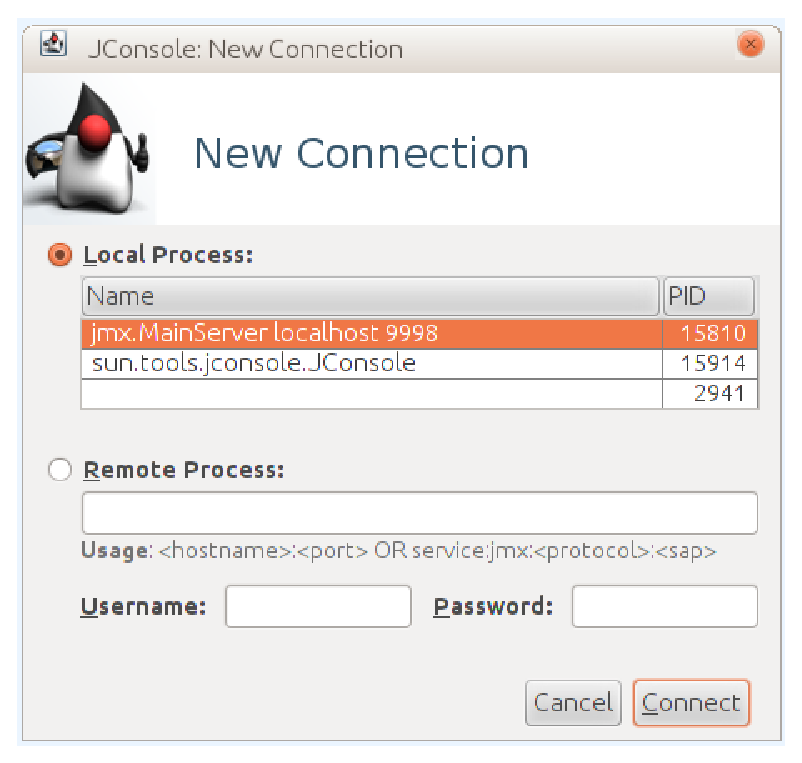
\includegraphics[scale=0.6]{graphics/jConsole.eps}
%\centering
% \caption[JConsole MBeans]{JConsole Angemeldete MBeans}
% \label{fig:JConsole}
%\end{figure}
%
%\begin{figure}[!htb]
%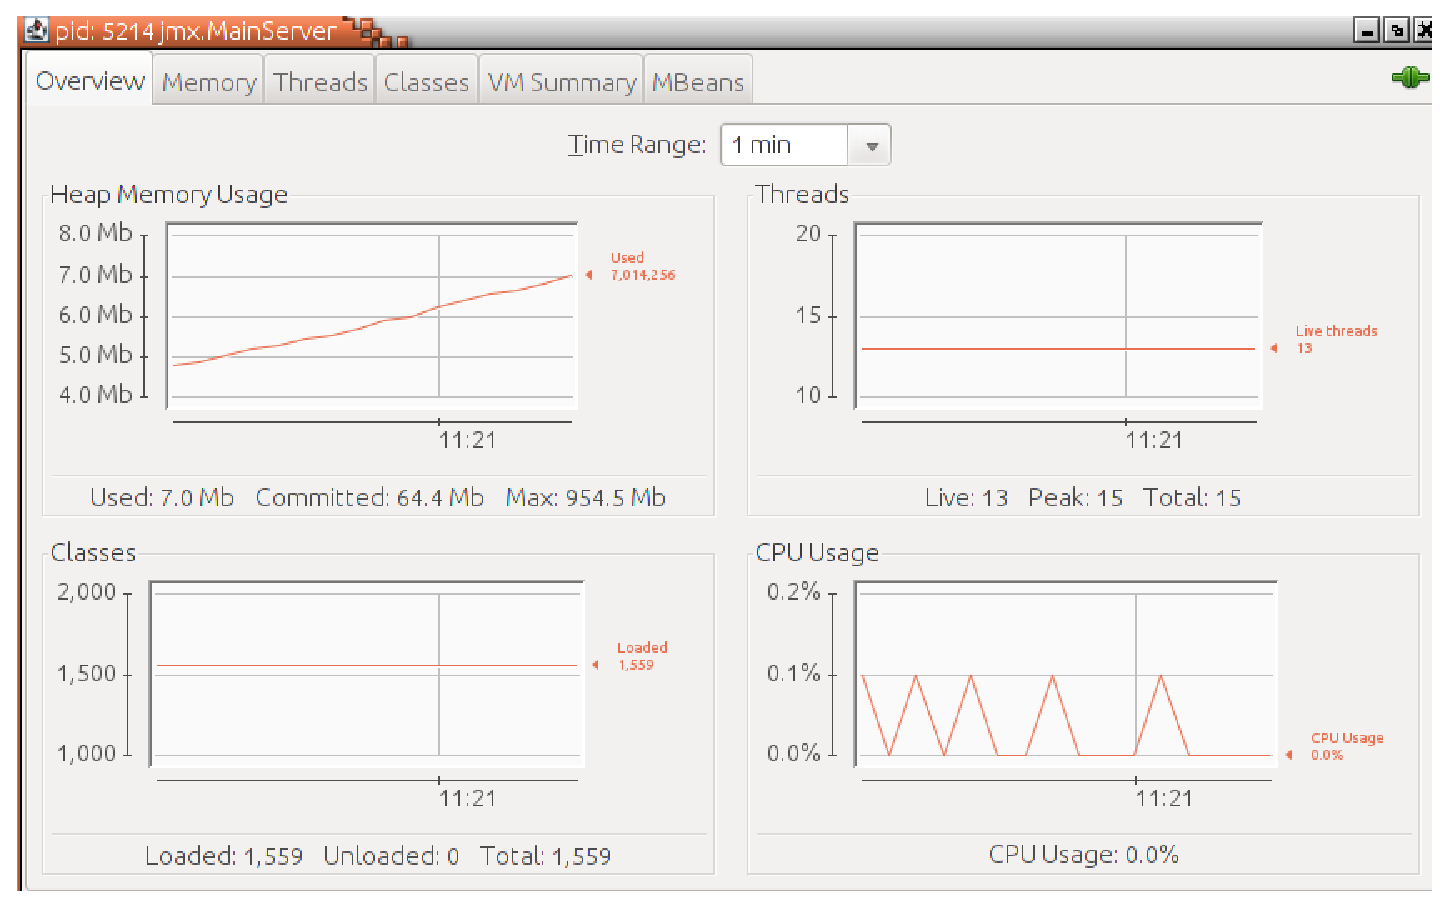
\includegraphics[scale=0.5]{graphics/jConsole2.eps}
%\centering
% \caption[JConsole Monitoring]{JConsole Monitoring}
% \label{fig:JConsole2}
%\end{figure}	
	
	\item Shell-Script: Eine andere Möglichkeit, um beispielsweise einen konsolenbasierten Client zu schrieben, ist durch die Verwendung von jmxterm\footnote{http://wiki.cyclopsgroup.org/jmxterm} gegeben. Daf\"ur ist lediglich ein einfaches Skript f\"ur den Verbindungsaufbau zum MBeanServer und der \"Ubergabe einer Ausf\"uhrungsliste notwendig. Die gew\"unschten Interaktionen werden unter Ber\"ucksichtigung einer gewissen Syntax in diese Liste\footnote{einfache Textdatei} geschrieben und dem Skript als Parameter \"ubergeben. Ein konkretes Beispiel wird im Kapitel Implementierung aufgezeigt.	
	
	\item Webbrowser: F\"ur die Agent-View \"uber einen Webbrowser bietet sich die Nutzung von JMXTools an. Neben dem MBeanServer muss die durch die Library bereitgestellte Klasse \courier{HtmlAdaptorServer} gestartet werden. Dieser wird zusätzlich ein Host und ein Port \"ubergeben. Mittels Webbrowser kann nun über den Host und den Port eine Verbindung zum \courier{MBeanServer} aufgebaut werden. Anschlie\ss end stehen die \courier{MBeans} zur Auswahl bereit. Die Operationen des gewählten \courier{MBeans} lassen sich nun \"uber den Webbrowser steuern.
	
%\begin{figure}[!htb]
%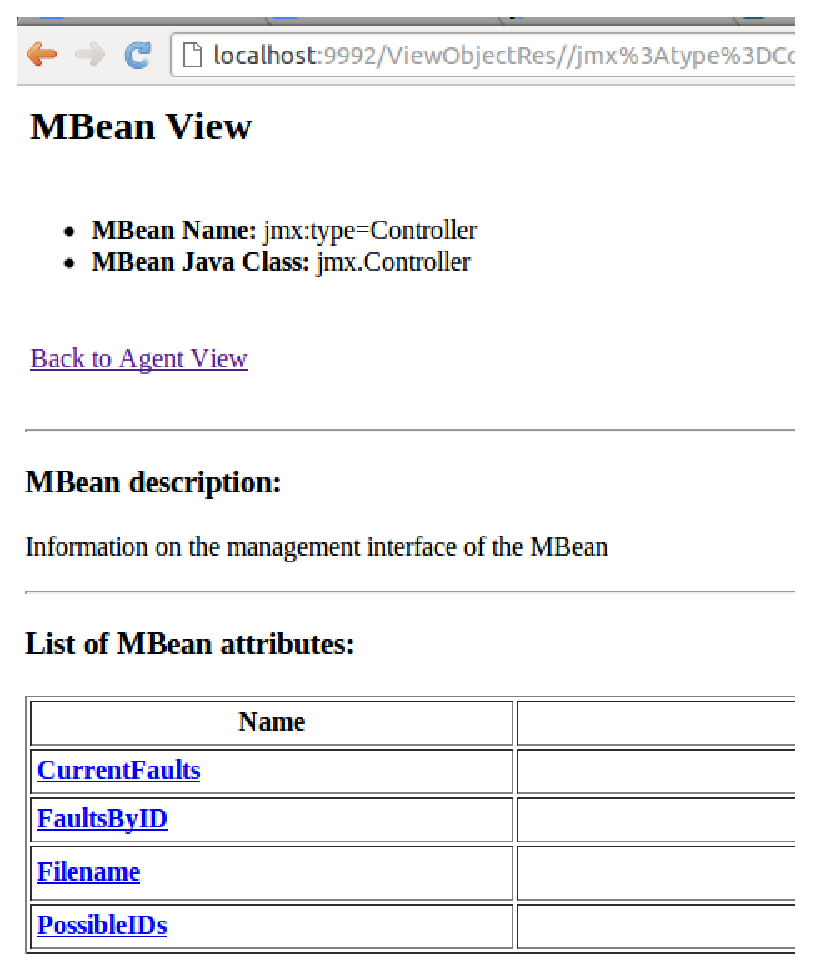
\includegraphics[scale=0.7]{graphics/htmlView.eps}
%\centering
% \caption[HtmlAdaptorServer]{HtmlAdaptorServer}
% \label{fig:HtmlAdaptorServer}
%\end{figure}		
	
	\item Java-Client: Java-Clients lassen sich ebenfalls über die \courier{ControllerMBean} Schnittstelle sehr leicht integrieren. Die Verbindung zum \courier{MBeanServer} wird \"uber RMI oder lokal aufgebaut. Ist die Verbindung erfolgreich können Variablen über \courier{Attribut}-Objekte gesetzt oder erfragt werden. Um die Methoden auszuführen ist ein \courier{Connection}-Objekt erforderlich.
\end{itemize}



%
\section{Sequenzieller Ablauf} 

Den zeitlichen Ablauf der Interaktion zwischen den Hauptklassen zeigt das Sequenzdiagramm aus Abbildung \ref{Sequenzdiagramm}. F\"ur die Nutzung des Programms ist die Anmeldung am MBean-Server als erster Schritt obligatorisch. Dieser stellt die Schnittstelle zum \courier{Controller} bereit, welcher alle erforderlichen Operationen f\"ur den Client verfügbar macht. Im Sequenzdiagramm aus Abbildung \ref{Sequenzdiagramm} ist zur Vereinfachung der Grafik die Verbindung zwischen Client und \courier{Controller} direkt eingezeichnet worden. \\
Nach der erfolgreichen Anmeldung am Server steht es dem Client frei welche Operation er ausf\"uhren m\"ochte. Auf der Zeitlinie aus Abbildung \ref{Sequenzdiagramm} folgt als erster Schritt eine Fehlerwertabfrage, um anhand der ID's neue Werte setzen zu können.\\
Im Anschluss wird die Default Fehlerinjektion vom Client gestartet. Der \courier{Controller} gibt den Aufruf zunächst an den \courier{StreamProcessor} weiter. Der \courier{StreamProcessor} liest die Daten ein und übergibt sie als Byteliste an ein \courier{Context}-Objekt. Die Klasse \courier{Context} wählt anhand der Fehlerwerte, in diesem Fall die Default Fehlerwerte im Quellcode, die erforderliche Strategie aus. Die Bytes werden mit Fehlern injiziert und zurück an den \courier{StreamProcessor} geschickt. 
Der Injektionsaufruf des \courier{Controllers} respektive des Clients wird nun vom \courier{StreamProcessor} durch das Schreiben der Daten in eine vorher angelegte Ausgabedatei zum Abschluss gebracht. \\
Eine Fehlerinjektion mit Streamwechsel ist in Abbildung \ref{Sequenzdiagramm} unter ``RunInjection mit Streamwechsel'' dargestellt. Zuerst wird ein anderer Ausgabestream gewählt. Diese Operation kann zeitlich auch später folgen, muss jedoch vor dem Injektionsaufruf ausgeführt werden. Danach wurden die Fehlerwerte neu gesetzt. Das Setzen der Fehlerwerte kann zu verschiedenen Ausnahmebehandlungen führen. Im Diagramm wurde eine falsche ID übergeben. Der Controller bekommt daraufhin bei der Modifikation der Annotationen eine Fehlermeldung übergeben, welche an den Client weitergereicht wird. Im Falle einer korrekten Übergabe der Fehlerwerte erhält der Controller einen modifizierten \courier{StreamProcessor}. Anschlie\ss end kann die Injektion vom Client veranlasst werden. Der Controller ruft an dieser Stelle die entsprechende Methode des modifizierten \courier{StreamProcessor} auf. Die weitere Verarbeitung geschieht ananlog zur Default Injektion.



\begin{figure}[!htb] 
\centering

\begin{sequencediagram}
\newthread{cl}{:Client}
\newinst[2]{contr}{:Controller}
\newinst[1]{fp}{:StreamProcessor}
\newinst[1]{conte}{:Context}
\newinst{ms}{:MainServer}

\begin{call}
	{cl}	{Anmeldung}{ms}{}
\end{call}

\begin{sdblock}{getCurrentFaults}{}

\begin{call}
	{cl}{gib Fehlerwerte}{contr}{aktuelle Fehlerwerte}
\end{call}

\end{sdblock}

\begin{sdblock}{RunInjection}{}

\begin{call}
	{cl}	{Injektion}{contr}{}
	\begin{call}
		{contr}{Injektion}{fp}{schreibe Daten}
		\begin{call}
			{fp}{übergabe Bytes}{conte}{injiz. Daten}
		\end{call}
	\end{call}
\end{call}

\end{sdblock}


\begin{sdblock}{RunInjection}{mit Streamwechsel}

\begin{messcall}
	{cl}{setze Ausgabestream}{contr}
\end{messcall}

\begin{call}
	{cl}	{setze Fehlerwerte}{contr}{Error ID falsch}
\end{call}

\begin{messcall}
	{cl}	{setze Fehlerwerte}{contr}{}
	\begin{call}
		{contr}{modif. StreamPr.}{fp}{}
	\end{call}
\end{messcall}


\begin{call}
	{cl}	{Injektion}{contr}{}
	\begin{call}
		{contr}{Injektion}{fp}{schreibe Daten}
		\begin{call}
			{fp}{übergabe Bytes}{conte}{injiz. Daten}
		\end{call}
	\end{call}
\end{call}
\end{sdblock}

\end{sequencediagram}

	\caption[Sequenzdiagramm]{Sequenzdiagramm}
 	\label{Sequenzdiagramm}
\end{figure}




%\newpage
%
%\begin{sequencediagram}
%\newthread[red]{r}{:Red}
%\newthread[green]{g}{:Green}
%\newthread[blue]{b}{:Blue}
%\tikzstyle{inststyle}+=[top color=yellow,bottom
%color=gray]
%\newinst{y}{:Yellow}
%\tikzstyle{inststyle}+=[bottom color=white,top
%color=white,rounded corners=3mm]
%\newinst{o}{:Rounded}
%\end{sequencediagram}
%
%\begin{sequencediagram}
%\newthread{ss}{:Client}
%\newinst{ctr}{:Controller}
%\newinst{ps}{:PhysicsServer}
%\newinst[1]{sense}{:FileProcessor}
%\begin{call}{ss}{Initialize()}{sense}{}
%\end{call}
%\begin{sdblock}{RunLoop}{Themainloop}
%\begin{call}{ss}{StartCycle()}{ctr}{}
%\begin{call}{ctr}{ActAgent()}{sense}{}
%\end{call}
%\end{call}
%\begin{call}{ss}{Update()}{ps}{}
%\begin{messcall}{ps}{PrePhysicsUpdate()}{sense}{state}
%\end{messcall}
%\begin{sdblock}{PhysicsLoop}{}
%\begin{callself}{ps}{PhysicsUpdate()}{}
%\end{callself}
%\end{sdblock}
%\begin{call}{ps}{PostPhysicsUpdate()}{sense}{}
%\end{call}
%\end{call}
%\begin{call}{ss}{EndCycle()}{ctr}{}
%\begin{call}{ctr}{SenseAgent()}{sense}{}
%\end{call}
%\end{call}
%\end{sdblock}
%\end{sequencediagram}


